\documentclass[t]{beamer}
\usepackage[utf8x]{inputenc}
\usepackage[ngerman]{babel}
\usepackage[T1]{fontenc}
\usepackage{textcomp}
\usepackage{subfigure}
\usepackage{graphicx}
\usepackage{fancyhdr}
\usepackage{tgpagella}
\usepackage[absolute,overlay]{textpos}
\usepackage{hyperref}
\usepackage{wasysym}
\usepackage{color}
\usepackage{tcolorbox}
\usepackage{tikz}

% ohne dieses Paket bekommt Carsten verpixelte Schrifen
\usepackage{lmodern}

\usetikzlibrary{decorations.pathreplacing}
\usetikzlibrary{calc}



\hypersetup{
colorlinks=true,
linkcolor=[rgb]{1, 1, 1}, %
urlcolor=[rgb]{.2, .2, .5} %
%allcolors=[rgb]{0, 0, 0} % schwarz
}

\usetheme{Dresden}
\useoutertheme{infolines}

% \setbeamerfont*{quote}{family=\sffamily}
% \addtobeamertemplate{quote begin}{}{\begin{tcolorbox}}
% \addtobeamertemplate{quote end}{\end{tcolorbox}}{}

\setbeamertemplate{navigation symbols}{} % we dont want navigation buttons

\title{Freie Software Freies Wissen Dresden}
\subtitle{Fund-Raising for Free Software - Thinking Big}
\author{\texttt{https://fsfw-dresden.de}}
\date{2018-12-29 (35C3)}



\addtobeamertemplate{frametitle}{}{%
  \begin{textblock*}{130mm}(.87\textwidth,8.4mm)
    
\includegraphics[width=2.25cm]{img-src/fsfw-logo.pdf}
  \end{textblock*}
}


\setbeamercolor{frametitle}{fg=black}

\synctex=1


\definecolor{softblue}{rgb}{0.3,0.3,.6}
\definecolor{lightblue}{rgb}{0.9,0.9,.95}
\newenvironment{cboxed}[1]
{\begin{tcolorbox}[colback=lightblue,colframe=softblue,title=#1]}
{\end{tcolorbox}}

\newcommand{\cst}[1]{{\usebeamercolor[fg]{structure}#1}}


% \includeonlyframes{p1}

\begin{document}

\begin{frame}[label=p1]
  \begin{center}%
\vspace*{-1em}

\includegraphics[width=4cm]{img-src/fsfw-logo-with-text}
\hspace{1cm}
\includegraphics[width=4cm]{img-src/gutschein-seite-1}\\
\vspace{1em}
\structure{\Large "`Fund-Raising for Free Software - Thinking Big"'}
  \end{center}
\end{frame}

%%%%%%%%%%%%%%%%%%%%%%%%%%%%%%%%%%%%%%%%%%%%%%%%%%%%%%%%%%%%%%%%%%%%%%%%%%%%%%%%

\begin{frame}[label=ol]{\usebeamercolor[fg]{structure}\color{fg}Overview}
  \begin{itemize}
  \item Who we are and what we do?
  \item Theses about free software for desktop usage
  \item Analysis of existing business models
  \item Idea: Combination-Model -- Selling Support Certificates
  \item How to proceed?
  \end{itemize}
\end{frame}




%%%%%%%%%%%%%%%%%%%%%%%%%%%%%%%%%%%%%%%%%%%%%%%%%%%%%%%%%%%%%%%%%%%%%%%%%%%%%%%%

\begin{frame}[label=ct1]{\usebeamercolor[fg]{structure}\color{fg}FSFW (1)}
Wer sind wir?
  \begin{itemize}
  \item Hochschulgruppe (gegründet 2014, ca. 10 P.)
  \item bisherige Projekte:
  \begin{itemize}
   \item Linux-Install-Party, Linux-Presentation-Day
   \item Verschlüsselungsgewinnspiel
   \item Monatliche \href{https://fsfw-dresden.de/sprechstunde}{Sprechstunde} (Textsatzsystem \LaTeX, UniStick, ...)
   \item Publikationen: \href{https://fsfw-dresden.de/programm}{Programmpapier}, \href{https://fsfw-dresden.de/blog}{Blogbeiträge}
   \item Workshops (\href{https://fsfw-dresden.de/git-ws}{git}, \href{https://fsfw-dresden.de/python-workshop}{python},
   \href{https://fsfw-dresden.de/gpg}{Mailverschlüsselung})
   \item Ringvorlesung: "`\href{https://fsfw-dresden.de/ringvorlesung}{Freie Software und Freies Wissen als Beruf}"'
   \smallskip
   \item UniStick mit freier Software
  \end{itemize}
  \end{itemize}
\end{frame}

%%%%%%%%%%%%%%%%%%%%%%%%%%%%%%%%%%%%%%%%%%%%%%%%%%%%%%%%%%%%%%%%%%%%%%%%%%%%%%%%

\begin{frame}[label=ct2]{\usebeamercolor[fg]{structure}\color{fg}FSFW (2)}
Warum machen wir das? $\rightarrow$ \textbf{Aus Überzeugung}\\[1cm]
  \begin{itemize}
  \item Überzeugung 1: freie und quelloffene Software ist (meist) besser
  \item[] technische/nicht technische Argumente
  \pause
  \bigskip
  \item Überzeugung 2: \textit{öffentlich finanzierte} wissenschaftliche Inhalte
  (AutorInnen, GutachterInnen) sollten nicht von \textit{öffentlich finanzierten}
  Bibliotheken für \textit{horrende Summen} von Zeitschriften-Verlagen gekauft werden müssen
  \end{itemize}
\end{frame}

%%%%%%%%%%%%%%%%%%%%%%%%%%%%%%%%%%%%%%%%%%%%%%%%%%%%%%%%%%%%%%%%%%%%%%%%%%%%%%%%


\begin{frame}[label=ct3,plain]{}

\vspace{1mm}
\begin{center}
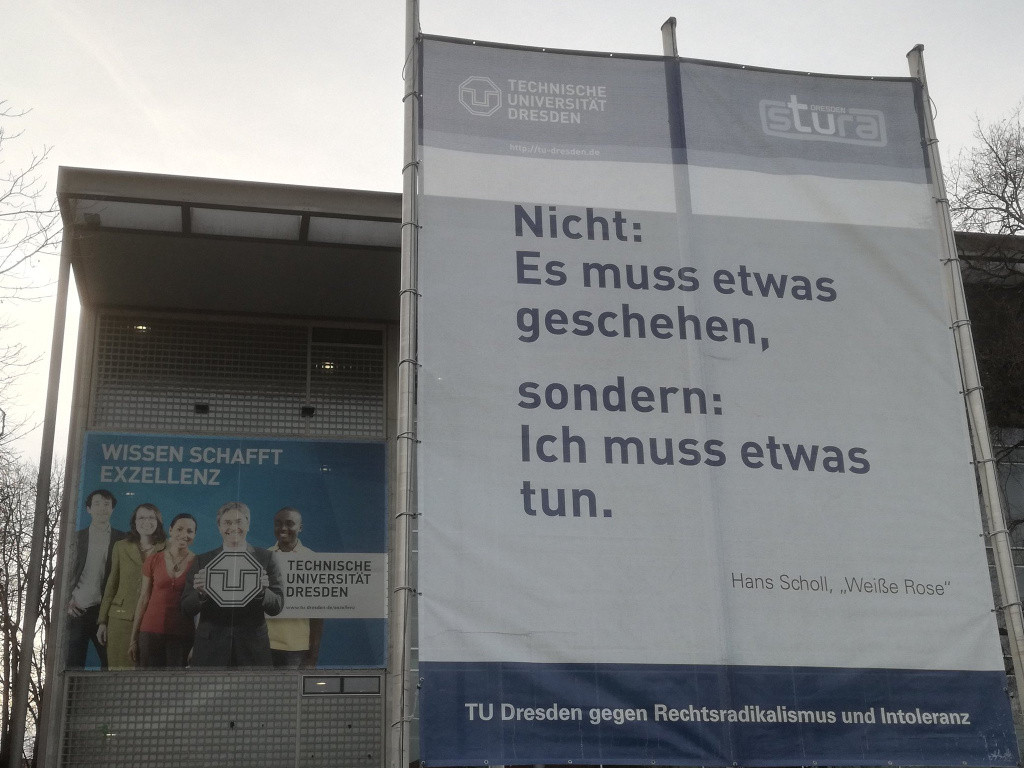
\includegraphics[width=1.05\textwidth]{img-src/tud-ich-muss-etwas-tun}
\end{center}
\end{frame}

%%%%%%%%%%%%%%%%%%%%%%%%%%%%%%%%%%%%%%%%%%%%%%%%%%%%%%%%%%%%%%%%%%%%%%%%%%%%%%%%
% content
%%%%%%%%%%%%%%%%%%%%%%%%%%%%%%%%%%%%%%%%%%%%%%%%%%%%%%%%%%%%%%%%%%%%%%%%%%%%%%%%
\newlength{\breite}


\begin{frame}[label=obs1]{\usebeamercolor[fg]{structure}Theses about free software for desktop usage}
\begin{enumerate}
\item There exist amazing products.
\pause
\medskip

\item Society would benefit from higher FOSS market share.
\pause
\medskip

\item FOSS has only a small market share.
\pause
\medskip

\item Many projects suffer from lacking resources,\\
user experience could be better with more ressources.
\pause
\bigskip
\bigskip

\item
\end{enumerate}


\begin{textblock*}{\textwidth}[0.,0.](10mm,55mm)
\setlength{\breite}{0.9\textwidth}
\only<+>{\includegraphics[width=\breite]{img-src/ffi_feedback_loop-01}}
\only<+>{\includegraphics[width=\breite]{img-src/ffi_feedback_loop-02}}

\end{textblock*}


\end{frame}

%%%%%%%%%%%%%%%%%%%%%%%%%%%%%%%%%%%%%%%%%%%%%%%%%%%%%%%%%%%%%%%%%%%%%%%%%%%%%%%%

\begin{frame}[label=obs2]{\usebeamercolor[fg]{structure}Observations}
Widespread ``classical'' business model:
\begin{itemize}
 \item Selling software usage rights or collected data
 \item Use revenues for development and PR
\end{itemize}
\pause
\smallskip
Not possible nor desired for FOSS

\pause
\medskip

{\usebeamercolor[fg]{structure}Why does the concept of ``Free Software'' work at all?}

\bigskip
People dedicate time and effort to FOSS-projects
\begin{itemize}
 \item driven by enthusiasm
 \item for fun
 \item to show their skills
 \item to learn new skills
 \bigskip

 \pause
 \item for money (raised by some exsiting FOSS business model)
\end{itemize}


\end{frame}

%%%%%%%%%%%%%%%%%%%%%%%%%%%%%%%%%%%%%%%%%%%%%%%%%%%%%%%%%%%%%%%%%%%%%%%%%%%%%%%%
%%%%%%%%%%%%%%%%%%%%%%%%%%%%%%%%%%%%%%%%%%%%%%%%%%%%%%%%%%%%%%%%%%%%%%%%%%%%%%%%

\begin{frame}[label=ol30]{}

\vspace{0.3\textheight}
\LARGE
\begin{center}
 \usebeamercolor[fg]{structure} Analysis of existing FOSS business models
\end{center}

\end{frame}

%%%%%%%%%%%%%%%%%%%%%%%%%%%%%%%%%%%%%%%%%%%%%%%%%%%%%%%%%%%%%%%%%%%%%%%%%%%%%%%%

\begin{frame}[label=obs3]{\usebeamercolor[fg]{structure}Existing FOSS Business Models}

Wikipedia: \href{https://en.wikipedia.org/wiki/Business_models_for_open-source_software}{18 business models}

\pause
\medskip
Not applicable\only<3->{/desired} for sustainable end-user software:
\begin{itemize}
 \item open sourcing on end-of-life,  dual-licensing, ...
 \pause
 \item selling support,  delayed open-sourcing, proprietary extensions
\end{itemize}

Remainder:

\begin{enumerate}
\item Selling of branded merchandise
\item Selling of certificates and trademark use
\item Partnership with funding organizations
\item Bounty driven development
\item Crowdfunding/reverse-bounty model
\item Advertising-supported software
\item Voluntary donations
\end{enumerate}


\end{frame}

%%%%%%%%%%%%%%%%%%%%%%%%%%%%%%%%%%%%%%%%%%%%%%%%%%%%%%%%%%%%%%%%%%%%%%%%%%%%%%%%

\begin{frame}[label=obs4]{\usebeamercolor[fg]{structure}``Voluntary Donations''}

\begin{itemize}
 \item contradict \textit{economic rationality}?
 \tikz[remember picture] \node[coordinate,yshift=0.7em] (A) {};

 \item express irrational altruism?
 \tikz[remember picture] \node[coordinate, xshift=9mm] (B) {};
\end{itemize}

\visible<2->{
\begin{tikzpicture}[overlay,remember picture]

  \draw[thick,decorate,decoration={brace,amplitude=5pt}]
        (A-|B) -- (B) node[midway, right=4pt] {\hspace{-1mm} No! {\footnotesize (For a sane definition of rationality)}};
\end{tikzpicture}
 } % end visible

\pause
\pause
\begin{cboxed}{Subjective Sidenote}
Model of \href{https://en.wikipedia.org/wiki/Homo_economicus}{homo economicus}
describes an extremely shortsighted psychopathic personality.
Much of the worlds problems originate in mistakenly propagating it as normative role model.
\end{cboxed}

\pause
Established examples of ``irrational spending''
\begin{itemize}
 \item Brand awareness and status consumption\\
 \item Future-oriented self-interest
\end{itemize}

\end{frame}

%%%%%%%%%%%%%%%%%%%%%%%%%%%%%%%%%%%%%%%%%%%%%%%%%%%%%%%%%%%%%%%%%%%%%%%%%%%%%%%%
%%%%%%%%%%%%%%%%%%%%%%%%%%%%%%%%%%%%%%%%%%%%%%%%%%%%%%%%%%%%%%%%%%%%%%%%%%%%%%%%

\begin{frame}[label=ol40]{}

\vspace{0.3\textheight}
\LARGE
\begin{center}
 \usebeamercolor[fg]{structure} Combination Model
\end{center}

\end{frame}

%%%%%%%%%%%%%%%%%%%%%%%%%%%%%%%%%%%%%%%%%%%%%%%%%%%%%%%%%%%%%%%%%%%%%%%%%%%%%%%%


\begin{frame}[label=cm10]{\cst{Combination Model (Overview)}}
\begin{textblock*}{\textwidth}[0.,0.](10mm,20mm)
\setlength{\breite}{0.9\textwidth}
\only<+>{\includegraphics[width=\breite]{img-src/ffi_principle-01}}
\only<+>{\includegraphics[width=\breite]{img-src/ffi_principle-02}}
\only<+>{\includegraphics[width=\breite]{img-src/ffi_principle-03}}
\only<+>{\includegraphics[width=\breite]{img-src/ffi_principle-04}}
\only<+>{\includegraphics[width=\breite]{img-src/ffi_principle-05}}
\only<+>{\includegraphics[width=\breite]{img-src/ffi_principle-06}}
\only<+>{\includegraphics[width=\breite]{img-src/ffi_principle-07}}
\only<+>{\includegraphics[width=\breite]{img-src/ffi_principle-08}}
\only<+>{\includegraphics[width=\breite]{img-src/ffi_principle-09}}
\bigskip
\only<1-5>{
\begin{itemize}
 \item<1-2> Challenge: several users want to fund several projects
 \item<3> Current situation: $n$-to-$m$ relationship $\rightarrow$ bad effort-benefit ratio
 \item<4-5> Proposal: specialized organizations\\
 Working title: ``Funding Freedom Initiative''
\end{itemize}
}
\only<6-8>{
\begin{itemize}
 \item<6-7> Users \textit{buy} ``Free Software Support Certificates''\\
  (and high quality merchandise material)
 \item<8> Users (optionally) state their preferred projects\\
 $\rightarrow$ Funds can be distributed accordingly
\end{itemize}
}
\only<9->{
\begin{itemize}
 \item<9> Interested projects register once and\\
 regularly publish activity reports
\end{itemize}
}

\end{textblock*}

\end{frame}


%%%%%%%%%%%%%%%%%%%%%%%%%%%%%%%%%%%%%%%%%%%%%%%%%%%%%%%%%%%%%%%%%%%%%%%%%%%%%%%%


\begin{frame}[label=cm20]{\cst{Combination Model (Details 1)}}
\vspace{10mm}
{\large \textbf{Why should people spend money on this?}}
\vspace{5mm}

\pause

\begin{enumerate}
\setlength\itemsep{1em}
 \item<+->  Support for Free Software ($\rightarrow$ \textit{Voluntary donation})
 \item<+->  Merchandise material ($\rightarrow$ \textit{Selling of branded merchandise})
 \item<+->  (Maybe) Privileged communication channel into the project team\\
 ($\rightarrow$ \textit{Bounty Driven Development}; $\rightarrow$ \textit{Selling support})
 \item<+-> (Maybe) Extra-features/no ads ($\rightarrow$ \textit{Advertising supported software})\\[1mm]
 \pause
 (Might be controversial $\rightarrow$ up to discussion)
\end{enumerate}

\end{frame}

%%%%%%%%%%%%%%%%%%%%%%%%%%%%%%%%%%%%%%%%%%%%%%%%%%%%%%%%%%%%%%%%%%%%%%%%%%%%%%%%
\begin{frame}[label=cm30]{\cst{Combination Model (Details 2)}}
\vspace{10mm}
{\large \textbf{How could the money be distributed?}}
\end{frame}

%%%%%%%%%%%%%%%%%%%%%%%%%%%%%%%%%%%%%%%%%%%%%%%%%%%%%%%%%%%%%%%%%%%%%%%%%%%%%%%%
\begin{frame}[label=cm40]{\cst{Combination Model (Details 3}}
\vspace{10mm}
{\large \textbf{How could the money be distributed?}}
\end{frame}

%%%%%%%%%%%%%%%%%%%%%%%%%%%%%%%%%%%%%%%%%%%%%%%%%%%%%%%%%%%%%%%%%%%%%%%%%%%%%%%%
\begin{frame}[label=cm50]{\cst{Combination Model (Details 4)}}
\vspace{10mm}
{\large \textbf{How could the money be distributed?}}
\end{frame}

%%%%%%%%%%%%%%%%%%%%%%%%%%%%%%%%%%%%%%%%%%%%%%%%%%%%%%%%%%%%%%%%%%%%%%%%%%%%%%%%
\begin{frame}[label=zf1]{\cst{Conclusion}}

\begin{textblock*}{\textwidth}[0.,0.](10mm,28mm)
\setlength{\breite}{0.9\textwidth}
\only<+>{\includegraphics[width=\breite]{img-src/ffi_feedback_loop-01}}
\only<+>{\includegraphics[width=\breite]{img-src/ffi_feedback_loop-02}}
\only<+->{\includegraphics[width=\breite]{img-src/ffi_feedback_loop-03}}

% \vspace{-10mm}\hspace{10mm}
\begin{center}
\visible<+->{Aim: establish positive feedback loop}
\end{center}
\end{textblock*}
\end{frame}

%%%%%%%%%%%%%%%%%%%%%%%%%%%%%%%%%%%%%%%%%%%%%%%%%%%%%%%%%%%%%%%%%%%%%%%%%%%%%%%%

\end{document}
